\documentclass[12pt]{article}

%_______packages___________________________________________________

% used to generate dummy text below
\usepackage{lipsum}

% increase space used for text on page
\usepackage[textheight=23cm,textwidth=17cm]{geometry}
\usepackage[compact]{titlesec}

%package for including figures 
\usepackage{graphicx}

%packages from the American Mathematical Society - good for symbols and various constructions
\usepackage{amsmath}
\usepackage{amssymb}

%package to include colour (color) in the text - can be convenient to highlight material, particularly when working on draft material
\usepackage{color}

%package for listing code, here Python 
\usepackage{listings}

%package to include urls
\usepackage[pdftex]{hyperref}
\hypersetup{
    colorlinks=true,
    urlcolor=cyan,
}

%_______commands to make the best use of space on a page________________
\parindent=0pt
\parskip=8.0pt
\baselineskip=12pt
\oddsidemargin=-0.5cm

%_______settings for listing computer code using the listings package________________

\definecolor{codegreen}{rgb}{0,0.6,0}
\definecolor{codegray}{rgb}{0.5,0.5,0.5}
\definecolor{codepurple}{rgb}{0.58,0,0.82}
\definecolor{backcolour}{rgb}{0.95,0.95,0.92}
\lstdefinestyle{mystyle}{
    backgroundcolor=\color{backcolour},   
    commentstyle=\color{codegreen},
    keywordstyle=\color{magenta},
    numberstyle=\tiny\color{codegray},
    stringstyle=\color{codepurple},
    basicstyle=\ttfamily\footnotesize,
    breakatwhitespace=false,         
    breaklines=true,                 
    captionpos=b,                    
    keepspaces=true,                 
    numbers=none,                    
    numbersep=5pt,                  
    showspaces=false,                
    showstringspaces=false,
    showtabs=false,                  
    tabsize=2}
\lstset{style=mystyle}

%_____use of macros to create convenient abbreviations, here for vectors

\newcommand{\av}{{\bf a}}
\newcommand{\bv}{{\bf b}}
\newcommand{\cv}{{\bf c}}     


%_______end of preamble and start the document proper________________


\begin{document}

\centerline{\LARGE{My Title}}
 
This is a template which you may find helpful in writing your report, though you do not need to use this, and can modify it as you wish.

\section{Section heading}
\label{sec:heading}

You can refer to text in other sections by using section labels,
e.g. you can see some example equations in section \ref{sec:heading}.

Here is an example of a simple equation. Equations are also labelled
so you can refer to them in the text, e.g. see equation
\eqref{eq:lv0}.

\begin{equation}
\label{eq:lv0}
\dot{r} = r(1 - g), \qquad \dot{g} = g(2 - r).
\end{equation}

\section{A few examples} 
\label{sec:examples}

Here are a few more equations and similar:
%
\begin{equation}
\mathcal{F} = \int_0^{10} e^{-x^2}\, \sin x \, dx , \quad
A = \begin{pmatrix} a & b \\ c & d \end{pmatrix} , \quad
{\bf v} = \begin{pmatrix} 1+\sqrt{2} \\ 1- \sqrt{2} \end{pmatrix}, 
\end{equation}
%
\begin{equation}
{\bf a} \times ( {\bf b} \times {\bf c} ) = ({\bf a}\cdot{\bf c} ) {\bf b} -  ({\bf a}\cdot{\bf b} ) {\bf c}, 
\end{equation}
%
\begin{equation}\frac{d^2 y}{dx^2} = \frac{x^2 + y^2}{x+y} , \quad
\log \epsilon(h)  = 2 \log h + \log C, \quad
\frac{\partial^2 \phi}{\partial t^2} = c^2 \frac{\partial^2 \phi}{\partial x^2} .
\end{equation}
%

If you find you are typing lots of things repetitiously then take a look at {\tt newcommand} constructions close to the top of the source file, and:
%
\begin{equation}
\av \times ( \bv \times \cv ) = ( \av \cdot \cv ) \bv -  ( \av \cdot \bv ) \cv, 
\end{equation}
%

Here is an example of incorporating a snippet of a Python script into the report (these should go in an appendix, after the main body of the report and the bibliography). 
  
\vspace{3mm}

\lstinputlisting[language=Python, firstline=6, lastline=16]{resonance-plot.py}

\vspace{3mm}

In figure \ref{fig:eg} we see a few nice graphics. It is better to let
any figures `float' and refer to them by their number in the main
text; then if they end up a page or two out from where they are
mentioned, this doesn't matter. If you try to place them precisely in
the text, it takes a lot of time and can be a losing battle with
\LaTeX. Note that you may need to crop pictures you bring in (if they
have white space around them), and note also that graphics may vary
for different types of computer and \LaTeX \, installations, so you
may need to experiment and do some searching online, where a lot of
\LaTeX \, help is available.
  
\begin{figure}
  \begin{center}
    (a)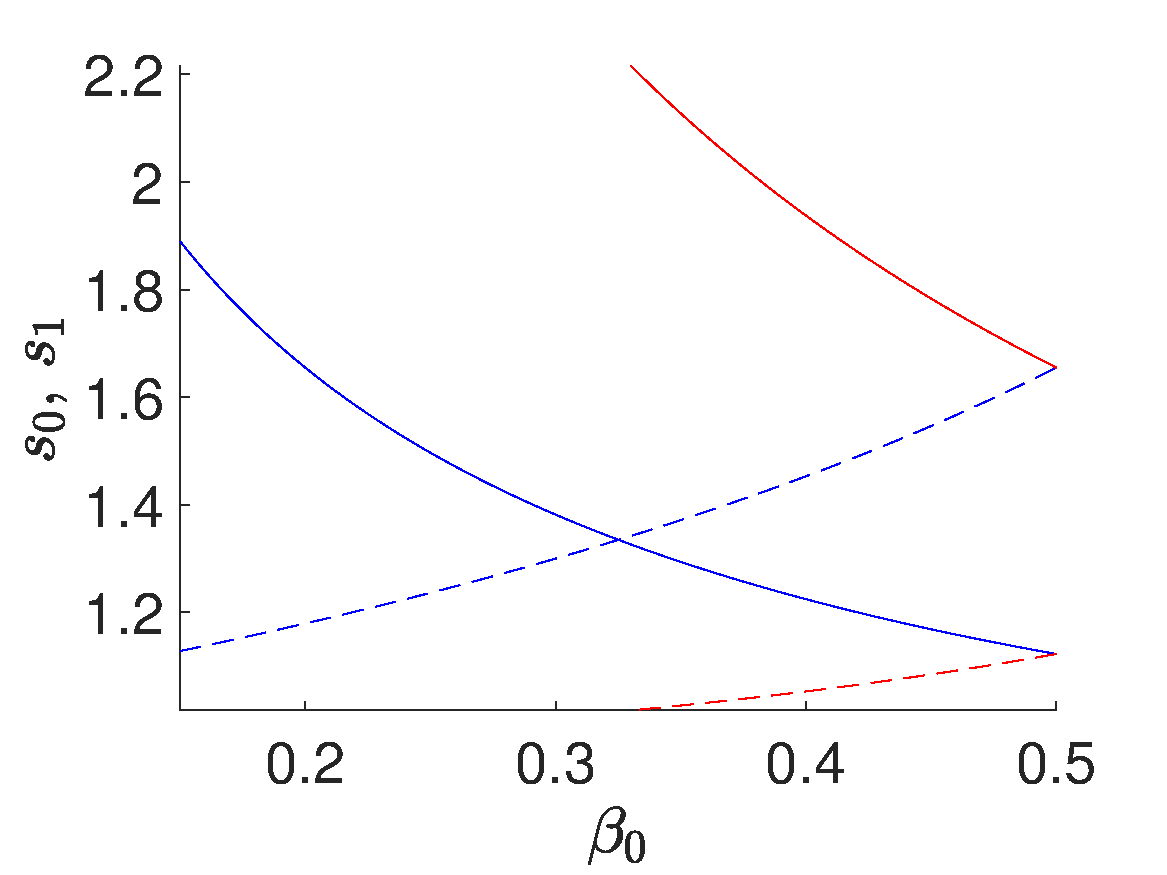
\includegraphics[scale=0.38]{fig-1a.pdf}
    (b)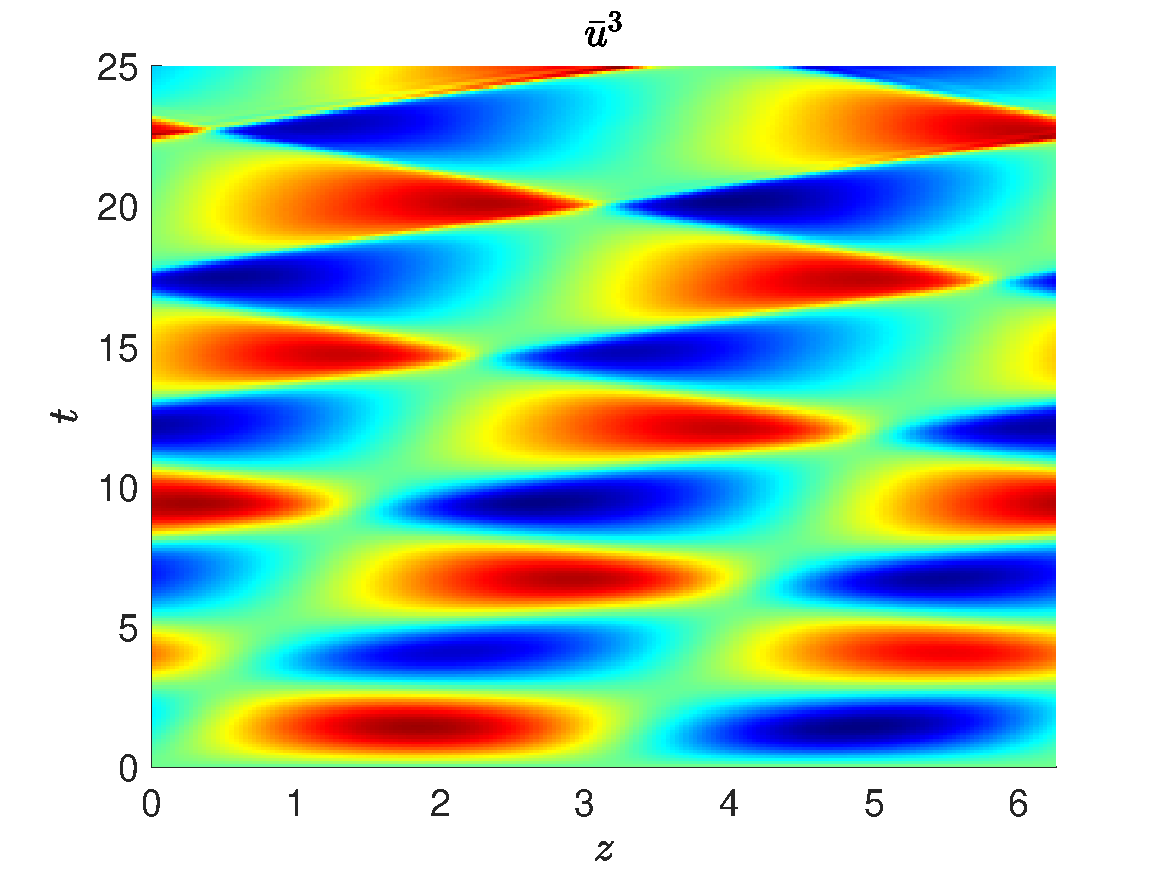
\includegraphics[scale=0.38]{fig-1b.pdf}\\
    \vspace{5mm}
    (c)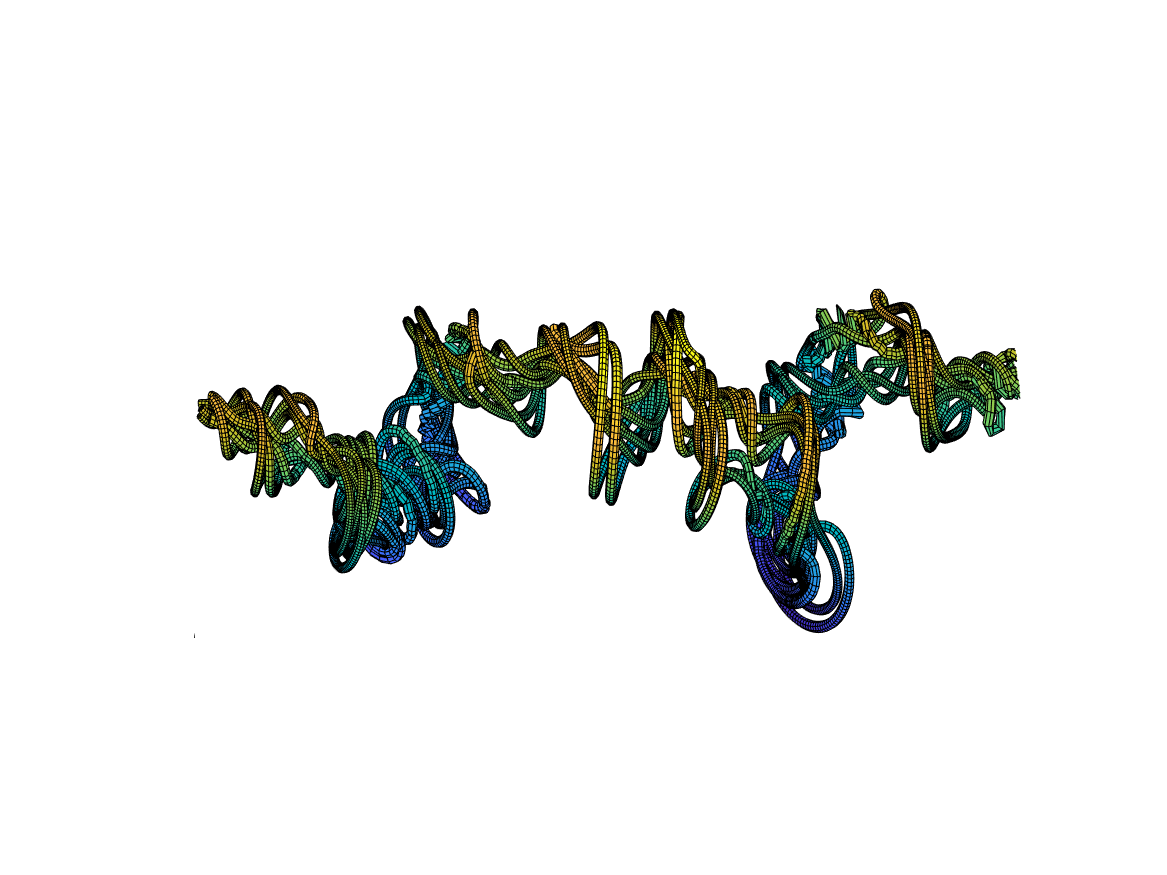
\includegraphics{fig-1c.pdf}
  \end{center}
  \caption{(a) a standard graph, (b) a colour picture using {\tt pcolor} in Python, and (c) helices wrapped around helices wrapped around helices.}
    \label{fig:eg}
\end{figure}

\section*{Bibliography}

There are many packages for doing bibliography and for
cross-referencing; however given that you are new to \LaTeX \, and the
report is not extensive I suggest you typeset bibliography without the
use of a package, for example as done here. Note the use of a
clickable link in reference 2.

[1] FitzHugh, R. 1961 Impulses and physiological states in theoretical models of nerve membrane. 
\emph{Biophys. J.} {\bf 1}, 445--466. 

[2] \url{https://en.wikipedia.org/wiki/Mary\_Cartwright}, Mary Cartwright, Wikipedia entry, accessed 17.2.26.

[3] Hodgkin, A.L. \& Huxley, A.F. 1952
A quantitative description of membrane current and its application to conduction and excitation in nerve.
\emph{J. Physiol.} {\bf 117}, 500--544. 


\appendix

\section{Appendix}

You can put your Python scripts and functions here, for example, again:

\lstinputlisting[language=Python]{linear_least_squares.py}


\end{document}

 
